%%%%%%%%%%%%%%%%%%%%%%%%%%%%%%%%%%%%%%%%%
% Beamer Presentation
% LaTeX Template
% Version 2.0 (March 8, 2022)
%
% This template originates from:
% https://www.LaTeXTemplates.com
%
% Author:
% Vel (vel@latextemplates.com)
%
% License:
% CC BY-NC-SA 4.0 (https://creativecommons.org/licenses/by-nc-sa/4.0/)
%
%%%%%%%%%%%%%%%%%%%%%%%%%%%%%%%%%%%%%%%%%

%----------------------------------------------------------------------------------------
%	PACKAGES AND OTHER DOCUMENT CONFIGURATIONS
%----------------------------------------------------------------------------------------

\documentclass[
11pt, % Set the default font size, options include: 8pt, 9pt, 10pt, 11pt, 12pt, 14pt, 17pt, 20pt
%t, % Uncomment to vertically align all slide content to the top of the slide, rather than the default centered
%aspectratio=169, % Uncomment to set the aspect ratio to a 16:9 ratio which matches the aspect ratio of 1080p and 4K screens and projectors
]{beamer}

\graphicspath{{Images/}{./}} % Specifies where to look for included images (trailing slash required)

\usepackage{booktabs} % Allows the use of \toprule, \midrule and \bottomrule for better rules in tables

%----------------------------------------------------------------------------------------
%	SELECT LAYOUT THEME
%----------------------------------------------------------------------------------------

% Beamer comes with a number of default layout themes which change the colors and layouts of slides. Below is a list of all themes available, uncomment each in turn to see what they look like.

%\usetheme{default}
%\usetheme{AnnArbor}
%\usetheme{Antibes}
%\usetheme{Bergen}
%\usetheme{Berkeley}
%\usetheme{Berlin}
%\usetheme{Boadilla}
\usetheme{CambridgeUS}
%\usetheme{Copenhagen}
%\usetheme{Darmstadt}
%\usetheme{Dresden}
%\usetheme{Frankfurt}
%\usetheme{Goettingen}
%\usetheme{Hannover}
%\usetheme{Ilmenau}
%\usetheme{JuanLesPins}
%\usetheme{Luebeck}
%\usetheme{Madrid}
%\usetheme{Malmoe}
%\usetheme{Marburg}
%\usetheme{Montpellier}
%\usetheme{PaloAlto}
%\usetheme{Pittsburgh}
%\usetheme{Rochester}
%\usetheme{Singapore}
%\usetheme{Szeged}
%\usetheme{Warsaw}

%----------------------------------------------------------------------------------------
%	SELECT COLOR THEME
%----------------------------------------------------------------------------------------

% Beamer comes with a number of color themes that can be applied to any layout theme to change its colors. Uncomment each of these in turn to see how they change the colors of your selected layout theme.

%\usecolortheme{albatross}
%\usecolortheme{beaver}
%\usecolortheme{beetle}
%\usecolortheme{crane}
%\usecolortheme{dolphin}
%\usecolortheme{dove}
%\usecolortheme{fly}
%\usecolortheme{lily}
%\usecolortheme{monarca}
%\usecolortheme{seagull}
%\usecolortheme{seahorse}
%\usecolortheme{spruce}
%\usecolortheme{whale}
%\usecolortheme{wolverine}

%----------------------------------------------------------------------------------------
%	SELECT FONT THEME & FONTS
%----------------------------------------------------------------------------------------

% Beamer comes with several font themes to easily change the fonts used in various parts of the presentation. Review the comments beside each one to decide if you would like to use it. Note that additional options can be specified for several of these font themes, consult the beamer documentation for more information.

\usefonttheme{default} % Typeset using the default sans serif font
%\usefonttheme{serif} % Typeset using the default serif font (make sure a sans font isn't being set as the default font if you use this option!)
%\usefonttheme{structurebold} % Typeset important structure text (titles, headlines, footlines, sidebar, etc) in bold
%\usefonttheme{structureitalicserif} % Typeset important structure text (titles, headlines, footlines, sidebar, etc) in italic serif
%\usefonttheme{structuresmallcapsserif} % Typeset important structure text (titles, headlines, footlines, sidebar, etc) in small caps serif

%------------------------------------------------

%\usepackage{mathptmx} % Use the Times font for serif text
%\usepackage{palatino} % Use the Palatino font for serif text

%\usepackage{helvet} % Use the Helvetica font for sans serif text
%\usepackage[default]{opensans} % Use the Open Sans font for sans serif text
%\usepackage[default]{FiraSans} % Use the Fira Sans font for sans serif text
%\usepackage[default]{lato} % Use the Lato font for sans serif text

%----------------------------------------------------------------------------------------
%	SELECT INNER THEME
%----------------------------------------------------------------------------------------

% Inner themes change the styling of internal slide elements, for example: bullet points, blocks, bibliography entries, title pages, theorems, etc. Uncomment each theme in turn to see what changes it makes to your presentation.

\useinnertheme{default}
%\useinnertheme{circles}
%\useinnertheme{rectangles}
%\useinnertheme{rounded}
%\useinnertheme{inmargin}

%----------------------------------------------------------------------------------------
%	SELECT OUTER THEME
%----------------------------------------------------------------------------------------

% Outer themes change the overall layout of slides, such as: header and footer lines, sidebars and slide titles. Uncomment each theme in turn to see what changes it makes to your presentation.

\useoutertheme{default}
%\useoutertheme{infolines}
%\useoutertheme{miniframes}
%\useoutertheme{smoothbars}
%\useoutertheme{sidebar}
%\useoutertheme{split}
%\useoutertheme{shadow}
%\useoutertheme{tree}
%\useoutertheme{smoothtree}

%\setbeamertemplate{footline} % Uncomment this line to remove the footer line in all slides
%\setbeamertemplate{footline}[page number] % Uncomment this line to replace the footer line in all slides with a simple slide count

%\setbeamertemplate{navigation symbols}{} % Uncomment this line to remove the navigation symbols from the bottom of all slides

%----------------------------------------------------------------------------------------
%	PRESENTATION INFORMATION
%----------------------------------------------------------------------------------------

\title[Short Title]{Full Presentation Title} % The short title in the optional parameter appears at the bottom of every slide, the full title in the main parameter is only on the title page

\subtitle{Optional Subtitle} % Presentation subtitle, remove this command if a subtitle isn't required

\author[James Cook \and Roald Amundsen]{Capt. James Cook \and Roald Amundsen} % Presenter name(s), the optional parameter can contain a shortened version to appear on the bottom of every slide, while the main parameter will appear on the title slide

\institute[UC]{the University of Cambridge \\ \smallskip \textit{james@LaTeXTemplates.com}} % Your institution, the optional parameter can be used for the institution shorthand and will appear on the bottom of every slide after author names, while the required parameter is used on the title slide and can include your email address or additional information on separate lines

%\date[\today]{International Symposium of Explorers \\ \today} % Presentation date or conference/meeting name, the optional parameter can contain a shortened version to appear on the bottom of every slide, while the required parameter value is output to the title slide

% PACKAGES
\usepackage[utf8]{inputenc}
\usepackage[T1]{fontenc}
\usepackage{lmodern}
\usepackage[english]{babel}
\usepackage{graphicx}%
\usepackage{multirow}%
\usepackage{amsmath,amssymb,amsfonts}%
\usepackage{amsthm}%
\usepackage{mathrsfs}%
\usepackage[title]{appendix}%
\usepackage{xcolor}%
\usepackage{textcomp}%
\usepackage{manyfoot}%
\usepackage{algorithm}%
\usepackage{algorithmicx}%
\usepackage{algpseudocode}%
\usepackage{listings}%
\usepackage{threeparttable}
\usepackage{dcolumn} %for stargazer in R
\usepackage{tikz}
\usepackage{verbatim}
%%%%
\usepackage{pgfplots}
\usepackage{pgfplotstable}
\usepackage{filecontents}

% BIBLIOGRAPHY %
\usepackage[natbib=true,style=authoryear,backend=bibtex,useprefix=true]{biblatex}
\addbibresource{bibliography.bib}
%optional
\setbeamercolor*{bibliography entry title}{fg=black}
\setbeamercolor*{bibliography entry location}{fg=black}
\setbeamercolor*{bibliography entry note}{fg=black}
\setbeamertemplate{bibliography item}{}
\renewcommand*{\bibfont}{\scriptsize}
%end styling

%Hypersetup for hyperlinks
\usepackage{hyperref}
\hypersetup{
	colorlinks=true,            
	linkcolor={red!50!black},
	citecolor={blue!50!black},
	urlcolor={blue!80!black}
}
\usepackage{float}

%%%%%=============================================================================%%%%
% color scheme
\newcommand{\red}[1]{\textcolor{red}{#1}}
\newcommand{\blue}[1]{\textcolor{blue}{#1}}
\newcommand{\green}[1]{\textcolor{green}{#1}}
\newcommand{\teal}[1]{\textcolor{teal}{#1}}

%%%%%=============================================================================%%%%

%\bibliography{sn-bibliography.bib}

\AtBeginSection[]{
	\begin{frame}
		\vfill
		\centering
		\begin{beamercolorbox}[sep=8pt,center,shadow=true,rounded=true]{title}
			\usebeamerfont{title}\insertsectionhead\par%
		\end{beamercolorbox}
		\vfill
	\end{frame}
}


\begin{document}
	\author{Quang-Thanh Tran}
	\title{A Short Course in \LaTeX}
	\subtitle{Inseikai Tohoku Bootcamp, Tohoku University}
	%\logo{}
	\institute{Summer Bootcamp}
	%\date{}
	%\subject{}
	%\setbeamercovered{transparent}
	%\setbeamertemplate{navigation symbols}{}
	
	\begin{frame}[plain]
		\maketitle %\titlepage
	\end{frame}
	
	%----------------------------------------------------------------------------------------
	%	TABLE OF CONTENTS SLIDE
	%----------------------------------------------------------------------------------------
	
	% The table of contents outputs the sections and subsections that appear in your presentation, specified with the standard \section and \subsection commands. You may either display all sections and subsections on one slide with \tableofcontents, or display each section at a time on subsequent slides with \tableofcontents[pausesections]. The latter is useful if you want to step through each section and mention what you will discuss.
	
	
	%----------------------------------------------------------------------------------------
	%	PRESENTATION BODY SLIDES
	%----------------------------------------------------------------------------------------
	
	%\section{Guide to \LaTeX}
	
	\begin{frame}
		\begin{figure}
			\centering
			\includegraphics[scale=0.4]{thomson.png}
			\includegraphics[scale=0.4]{thomson_copy.png}
			\caption{From Thomson's \href{https://www.amazon.co.jp/s?k=9780262201339}{A Guide for the Young Economist}}
		\end{figure}
	\end{frame}
	
	
	\begin{frame}{Installing \LaTeX}
		\begin{itemize}
			\item What is \LaTeX?
			\begin{itemize}
				\item Text Editor for researchers.
				\item Type in a source code -- render a document in PDF.
			\end{itemize}
			\item Why \LaTeX ?
			\begin{itemize}
				\item It's \red{free}, light, indestructible.
				\item It handles long documents well
				\item It supports math \& graphs (with \href{https://www.overleaf.com/learn/latex/LaTeX_Graphics_using_TikZ\%3A_A_Tutorial_for_Beginners_(Part_1)\%E2\%80\%94Basic_Drawing}{TikZ}), citations, cross-referencing.
			\end{itemize}
			\item Install a distribution package
			\begin{itemize}
				\item Windows: use \href{https://miktex.org/download}{MikTeX}
				\item Mac: use \href{https://www.tug.org/mactex/}{MacTeX}. Homebrew: use \texttt{brew install --cask mactex}
			\end{itemize}
			\item Install a TeX editor
			\begin{itemize}
				\item \href{https://www.texifier.com/}{Texifier}: \$40 (perpetual), very fast, WYSIWYG, Grammarly-enabled
				\item \href{https://www.texstudio.org/}{TeXstudio}: free, okay fast, not WYSIWYW, PDF is navigatable.
				\item \href{https://obsidian.md/}{Obsidian} or VScode: free, fast, handy if you want vanilla \LaTeX.
				\item \href{https://www.overleaf.com/}{Overleaf}: free, online, not fast, support 2-author collaboration.
			\end{itemize}
		\end{itemize}
	\end{frame}
	
	\section{The Basics}
	\begin{frame}{Structures}
		\begin{itemize}
			\item Preambles
				\begin{itemize}
					\item Define the document class and customized commands 
					
					\colorbox{yellow}{\texttt{\textbackslash documentclass[11pt,a4paper]\{article\}}}
					\item Declare packages to use \colorbox{yellow}{\texttt{\textbackslash usepackage\{amsmath\}}}
					\item Declare title, authors, etc. \colorbox{yellow}{\texttt{\textbackslash author\{\}, \textbackslash title\{\}}}
				\end{itemize}
			\item Content
			\begin{itemize}
					\item Make title by typing \colorbox{yellow}{\texttt{\textbackslash maketitle}}, ToC by \colorbox{yellow}{\texttt{\textbackslash tableofcontents}}.
					\item Special characters such as \colorbox{yellow}{\texttt{\_, \%, \$}} and commands start with \texttt{\textbackslash}
					\item The whole content must be nested between \blue{\texttt{\textbackslash begin\{document\}}} and \blue{\texttt{\textbackslash end\{document\}}}. To make new page \colorbox{yellow}{\texttt{\textbackslash newpage}}.
					\item Use \blue{\texttt{\textbackslash section\{<name>\}}, \texttt{\textbackslash subsection\{<name>\}} , \texttt{\textbackslash subsubsection\{<name>\}} } for automatic sectioning.
					\item use \% to make comments. (which are not rendered)
				\end{itemize}
			\item Bibliography
			\begin{itemize}
					\item ``Author(year)" -- use \texttt{\textbackslash \colorbox{yellow}{citet\{\}}}, for ``(Author,year)" -- use \colorbox{yellow}{\texttt{\textbackslash citep\{\}}}
					\item to print bibliography, use \colorbox{yellow}{\texttt{\textbackslash bibliography\{file.bib\}}} at the end.
			\end{itemize}
		\end{itemize}
	\end{frame}
	
	\begin{frame}{Math}
		\begin{itemize}
			\item Basics
			\begin{itemize}
						\item inline: nested between \$ \$ or \texttt{\textbackslash [} \texttt{\textbackslash ]}, for example: 
						
						\texttt{\$y\_i = x\^{}\{-1\}\_i + a\^{}2\$} produces $y_i = x^{-1}_i + a^2$
						\item single: nested between \texttt{\textbackslash begin\{equation\}} and \texttt{\textbackslash end\{equation\}}
						\item alignable: nested between \texttt{\textbackslash begin\{align\}} and \texttt{\textbackslash end\{align\}}
						\item lines are separated by \textbackslash\textbackslash, aligned by putting \& at the alignment.
						\item Putting a \texttt{*} at the commands \texttt{\textbackslash begin\{align*\}} -- \texttt{\textbackslash end\{align*\}}, all maths will be unnumbered. Use \texttt{\textbackslash nonumber} to turn it off individually.
					\end{itemize} 
			\item Syntax:
			\begin{itemize}
				\item fractions: \texttt{\textbackslash frac\{a\}\{b\}} $\to$ $\frac{a}{b}$
				\item superscript: \texttt{a\^{}b} $\to a^b$, subscript: \texttt{a\_ b} $\to a_b$
				\item Greeks: \texttt{\textbackslash gamma} $\to \gamma$, \texttt{\textbackslash Gamma} $\to \Gamma$
				\item For more commands, check: \href{https://www.cmor-faculty.rice.edu/~heinken/latex/symbols.pdf}{\LaTeX \ Mathematical Symbols}
			\end{itemize}
			\item Referencing
			\begin{itemize}
				\item to label an equation, use \texttt{\textbackslash label\{eq\_foc\}}
				\item to reference that equation, use \texttt{\textbackslash eqref\{eq\_foc\}}
				\item you can label sections or theorems and reference them with \texttt{\textbackslash ref\{sec\}}
			\end{itemize}
		\end{itemize}
	\end{frame}
	
	\begin{frame}{Figures}
		To add a figure
		\begin{itemize}
			\item Make sure the figure is in the same path as the .tex file.
			\item Use the following code \\
			\texttt{\textbackslash begin\{figure\}}[ht] \\
			\texttt{\textbackslash centering} \\
			\texttt{\textbackslash includegraphics[scale=0.5]\{figure.png\}} \\
			\texttt{\textbackslash caption\{A Figure of a Cat.\}} \\
			\texttt{\textbackslash label\{fig:cat\}} \\
			\texttt{\textbackslash end\{figure\}}
			\item Options: \texttt{\textbackslash includegraphics[width=0.5\textbackslash textwidth,right]\{figure\}}
			\item Positioning: [h] \textit{here}, [t] \textit{top}, [b] \textit{bottom}, [H] \textit{here!} (need \texttt{float})
		\end{itemize}
	\end{frame}
	
	\begin{frame}{Tables}
		Tables are extremely easy \\
		
		\texttt{\textbackslash begin\{table\}}[ht] \\
		\texttt{\textbackslash centering} \\
		\texttt{\textbackslash begin\{tabular\}\{ c | c | c \}} $\blacktriangleleft$ \blue{3 columns, centered, with | between} \\
			\texttt{ \textbackslash toprule  } \\
			\texttt{ variable \& value \& meaning \textbackslash \textbackslash } \\
			\texttt{ \textbackslash midrule  } \\
			\texttt{ \$\textbackslash alpha\$ \& 0.3 \& capital share \textbackslash \textbackslash } \\
			\texttt{ r \& 1.05 \& interest rate \textbackslash \textbackslash } \\
			\texttt{ \textbackslash bottomrule } \\
			\texttt{\textbackslash end\{tabular\}}
			\texttt{\textbackslash caption\{Regression result\}} \\
			\texttt{\textbackslash label\{tab:result\}} \\
			\texttt{\textbackslash end\{table\}}
	\end{frame}
	
	
	\begin{frame}
		Rendered: (I disabled the | between columns)
		\begin{table}
			\centering
			\begin{tabular}{c  c  c}
				\toprule 
				variable & value & meaning \\
				\midrule
				$\alpha$ & 0.3 & capital share \\
				r & 1.05 & interest rate \\
				\bottomrule
			\end{tabular}
			\caption{Parameters}
		\end{table}
		You can convert results in R, Stata, and Python to copy-paste in \LaTeX \\
		(just search it on Google)
	\end{frame}
	
	\begin{frame}{Exercises}
		\begin{itemize}
			\item Try it yourself by rendering the code uploaded \href{https://github.com/thanhqtran/tohoku_bootcamp/tree/main/tex_guide}{here} on your computer.
			You can find it at the boot camp's site \url{https://github.com/thanhqtran/tohoku_bootcamp/tree/main}
			
			\item Exercises: See \href{https://guides.nyu.edu/LaTeX/exercises}{\url{https://guides.nyu.edu/LaTeX/exercises}}
			
			Today, do 
			\begin{itemize}
				\item Exercise 4: Creating Sections and Referencing Equation
				\item Exercise 5: Creating Matrix Equations
				\item [optional] Exercise 6: Tables and Figures
				\item [optional] Exercise 7: Bibliography
				\item [optional] Additional Exercises: \texttt{\textbackslash newcommand}
			\end{itemize}
			
			\item For this class, I encourage you to type everything in \LaTeX{} after you finish solving with pen and paper.
			\item You can use \href{https://github.com/thanhqtran/tohoku_bootcamp/blob/main/tex_guide/template.tex}{this template}, it has everything you need.
			
		\end{itemize}
	\end{frame}
	
	\section{Notes}
	
	\begin{frame}{todonotes}
		\begin{itemize}
			\item Put this in preamble: \texttt{\textbackslash usepackage\{todonotes\}}
			\item To comment, type: \texttt{\textbackslash todo\{content\}}  after some words. This option will push the comment to the paper margin.
			\item You can change color or insert drop shadow \texttt{\textbackslash todo[color=green!40, shadow]\{content\}} or \texttt{noshadow}
			\item If you want an inline comment, type \texttt{\textbackslash todo[inline, inlinewidth=5cm]\{content\}}
			\item To add author, add \texttt{\textbackslash todo[author=John]\{content\}}
			\item Documentation: \url{https://ftp.kddilabs.jp/CTAN/macros/latex/contrib/todonotes/todonotes.pdf}
		\end{itemize}
	\end{frame}
	
	\begin{frame}{Example}
		\begin{figure}
			\includegraphics[scale=0.4]{note.png}
		\end{figure}
	\end{frame}
	
	\section{Plots}
	\begin{frame}{TikZ}
		You can plot directly or import data from an outside file to make plots!
		
		\begin{itemize}
		\item Preamble: \\
		
		\texttt{\textbackslash usepackage\{tikz\} } \\
		\texttt{\textbackslash usepackage\{tikzscale\}} \\
		\texttt{\textbackslash usetikzlibrary\{arrows,calc, automata, patterns, positioning, shapes.geometric, decorations.pathreplacing,decorations.markings\}}
		
		\item For more tikz plots related to economics, see:
		\url{https://web.archive.org/web/20221023220457/https://sites.google.com/site/kochiuyu/Tikz}
		
		\item If you want to know why we prefer to plot directly (or export an image to .pdf or .svg), try to zoom in a vector image vs a normal image (raster). The raster images become blurred or pixelated, while the vector image does not lose any sharpness or quality. 
		\end{itemize}
	\end{frame}
	
	\begin{frame}{pgfplot}
		\begin{itemize}
		\item Preamble: \\
		
		\texttt{\textbackslash usepackage\{pgfplots\} } \\
		\texttt{\textbackslash usepackage\{pgfplotstable\}} \\
		\texttt{\textbackslash usepackage\{filecontents\}}
		
		\item For guidance, see:
		\url{https://www.overleaf.com/learn/latex/Pgfplots_package}
		\end{itemize}
		Example:
		\begin{figure}
		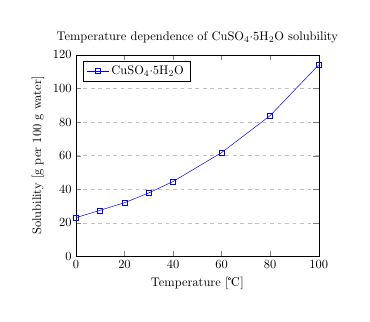
\begin{tikzpicture}[scale=0.45]
\begin{axis}[
    title={Temperature dependence of CuSO\(_4\cdot\)5H\(_2\)O solubility},
    xlabel={Temperature [\textcelsius]},
    ylabel={Solubility [g per 100 g water]},
    xmin=0, xmax=100,
    ymin=0, ymax=120,
    xtick={0,20,40,60,80,100},
    ytick={0,20,40,60,80,100,120},
    legend pos=north west,
    ymajorgrids=true,
    grid style=dashed,
]

\addplot[
    color=blue,
    mark=square,
    ]
    coordinates {
    (0,23.1)(10,27.5)(20,32)(30,37.8)(40,44.6)(60,61.8)(80,83.8)(100,114)
    };
    \legend{CuSO\(_4\cdot\)5H\(_2\)O}
    
\end{axis}
\end{tikzpicture}
	\end{figure}
	\end{frame}
	
	
	\begin{frame}{Example 1}
    \begin{columns}[onlytextwidth] % Make columns fit within the text width
        \begin{column}{0.4\textwidth}
            \texttt{\textbackslash begin\{tikzpicture\}} \\
			\texttt{\textbackslash begin\{axis\}[} \\
    		\texttt{axis lines = left,} \\
    		\texttt{xlabel = \(x\),} \\
    		\texttt{ylabel = {\(f(x)\)},} \\
			\texttt{]} \\

			\texttt{\textbackslash addplot [} \\
    		\texttt{domain=-10:10,} \\
    		\texttt{samples=100,} \\
    		\texttt{color=red,} \\
		\texttt{]} \\
		\texttt{\{ \$ x\^{}2 - 2*x - 1\$ \};} \\
		\texttt{\textbackslash addlegendentry\{\ \$ x\^{}2 - 2x - 1\$\}} \\

		\texttt{\textbackslash end\{axis\}} \\
		\texttt{\textbackslash end\{tikzpicture\}} 
        \end{column}
        
        \begin{column}{0.6\textwidth}
            \begin{figure}
                \begin{tikzpicture}
                    \begin{axis}[
                        axis lines = left,
                        xlabel = \(x\),
                        ylabel = {\(f(x)\)},
                        width=0.7\columnwidth, % Adjust the width as needed
                    ]
                    \addplot [
                        domain=-10:10,
                        samples=100,
                        color=red,
                    ]
                    {x^2 - 2*x - 1};
                    \addlegendentry{\(x^2 - 2x - 1\)}
                    \end{axis}
                \end{tikzpicture}
            \end{figure}
        \end{column}
    \end{columns}
    
	\end{frame}
	
		\begin{frame}{Example 2}
    \begin{columns}[onlytextwidth] % Make columns fit within the text width
        \begin{column}{0.7\textwidth}
            \texttt{\textbackslash begin\{tikzpicture\}} \\
\texttt{\textbackslash path [fill=yellow] (0,0) -- (0,5) to [out=-80, in=160} \\
\texttt{(3,.8) -- (3,0) -- (0,0);} \\
\texttt{\textbackslash draw [<->] (0,6) node [left] \{\ \$ P \$ \} -- (0,0)} \\
\texttt{node [below left] \{(0,0)\} -- (7,0) node [below] \{\ \$ Q \$ \};} \\
\texttt{\textbackslash draw [ultra thick, dashed] (0,.8) node [left] \{\ \$ P\^{}*=.8\$ \} -- (3,.8)} \\
\texttt{-- (3,0) node [below] \{\ \$ Q\^{}*=3\$ \};} \\
\texttt{\textbackslash draw [fill] (3,.8) circle [radius=.1];} \\
\texttt{\textbackslash draw [thick] (0,5) to [out=-80, in=160] (3,.8) to} \\
\texttt{[out=-20, in=175] (6,0);} \\
\texttt{\textbackslash end\{tikzpicture\}}

        \end{column}
        
        \begin{column}{0.3\textwidth}
            \begin{figure}
                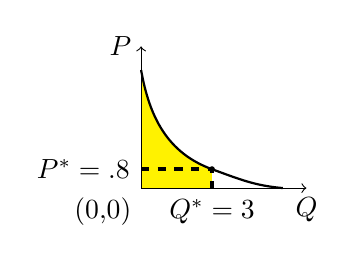
\begin{tikzpicture}[scale=0.3]
\path [fill=yellow] (0,0) -- (0,5) to [out=-80, in=160]
(3,.8) -- (3,0) -- (0,0);
\draw [<->] (0,6) node [left] {$P$} -- (0,0)
node [below left] {(0,0)} -- (7,0) node [below] {$Q$};
\draw [ultra thick, dashed] (0,.8) node [left] {$P^*=.8$} -- (3,.8)
-- (3,0) node [below] {$Q^*=3$};
\draw [fill] (3,.8) circle [radius=.1];
\draw [thick] (0,5) to [out=-80, in=160] (3,.8) to
[out=-20, in=175] (6,0);
\end{tikzpicture}
            \end{figure}
        \end{column}
    \end{columns}
    
	\end{frame}
	
	\section{Slides}
	
	\begin{frame}{Syntax}
	\begin{itemize}
		\item You document will be \colorbox{yellow}{\texttt{\textbackslash documentclass\{beamer\}}}
		\item You can use various themes. \colorbox{yellow}{\texttt{\textbackslash usetheme\{\}}}. This presentation uses \texttt{CambridgeUS}
		\item To create a new slide, use \\
		\colorbox{yellow}{\texttt{\textbackslash begin\{frame\}}} \\
		\colorbox{yellow}{\texttt{\textbackslash frametitle\{Title\}}} \\
		\colorbox{yellow}{content} \\
		\colorbox{yellow}{\texttt{\textbackslash end\{frame\}}}
		\item To highlight important text \\
		\colorbox{yellow}{\texttt{\textbackslash begin\{block\}}} \\
		\colorbox{yellow}{content} \\
		\colorbox{yellow}{\texttt{\textbackslash end\{block\}}} \\
		you can use \texttt{alertblock} instead of \texttt{block}
	\end{itemize}
	\end{frame}
	
	\begin{frame}{Beamer example}
		\begin{figure}
			\includegraphics[scale=0.25]{beam.png}
		\end{figure}
	\end{frame}
	
	\section{CV}
	\begin{frame}{Make professional CV}
		\begin{itemize}
		\item Shopping for templates here \url{https://www.latextemplates.com/cat/curricula-vitae}
		
		\item But for academics, consider this one
		
		\url{https://www.stat.berkeley.edu/~paciorek/computingTips/Latex_template_creating_CV_.html}
		
		\end{itemize}
	\end{frame}
	
	\begin{frame}{Example}
		\begin{figure}[ht]
			\includegraphics[scale=0.3]{cv_example.png}
			\caption{\tiny \url{https://www.stat.berkeley.edu/~paciorek/files/cv/paciorek-cv.pdf} }
		\end{figure}
	\end{frame}
	
	\begin{frame}{Host CV online}
		\begin{enumerate}
			\item Make a Git account, then a public repo. \colorbox{yellow}{user/repo/}
			\item Upload the CV in pdf format, say \colorbox{yellow}{cv.pdf} at branch \colorbox{yellow}{main}
			\item Copy the permanent link to the file \\
			 \colorbox{yellow}{\url{https://raw.githubusercontent.com/user/repo/main/cv.pdf}}
			\item Add google doc preview before the link \\
			\tiny \colorbox{yellow}{\red{https://docs.google.com/viewer?url=}\url{https://raw.githubusercontent.com/user/repo/main/cv.pdf}}
		\end{enumerate}
		Try: \url{https://docs.google.com/viewer?url=https://raw.githubusercontent.com/thanhqtran/tohoku_bootcamp/main/summer2023/math/summer_math.pdf}
	\end{frame}
	
	\section{Pandoc}
	\begin{frame}{Convert .tex to .docx}
		\begin{enumerate}
			\item Install \texttt{pandoc}: \url{https://pandoc.org/installing.html}
			\item Go to command center/ terminal and type \\
			\colorbox{yellow}{\texttt{pandoc mydoc.tex -o mydoc.docx}}
			\item To convert with citations \\
			\colorbox{yellow}{\texttt{pandoc mydoc.tex --bibliography=myref.bib -o mydoc.docx}}
			\item You can turn on cross-referencing
			\colorbox{yellow}{\texttt{pandoc mydoc.tex --filter pandoc-crossref --bibliography=myref.bib -o mydoc.docx}}
		\end{enumerate}
	\end{frame}
	
	%----------------------------------------------------------------------------------------
	%	BIB
	%----------------------------------------------------------------------------------------

	
		
	
	
	
	
\end{document}